Om de haalbaarheid van mijn onderzoek na te gaan, heb ik eerst een pilot study
gedaan. Ik heb hiervoor de virtuele omgeving ontworpen, en dan enkele
proefpersonen gevraagd deze met toetsenbord en muis te doorlopen.

\section{Virtuele Omgeving}
Voor dit onderzoek heb ik een virtuele omgeving ontworpen met meer dan 48m$^2$
aan bewandelbare ruimte, de proefpersoon kan deze omgeving volledig verkennen en
toch in een 12m$^2$ tracking area blijven. Deze virtuele omgeving bestaat uit 
een lange gang met drie kantoren en een uitgang er direct aan verbonden. De 
kantoren zijn zo ontworpen dat het mogelijk is om de deur te verplaatsen wanneer 
de proefpersoon deze niet in het zicht heeft. De gang zelf is 1 meter breed met 
een arbitraire lengte zodat deze oneindig lang lijkt. De kantoren zijn allemaal 
ontworpen om 3m x 3m te zijn. 

\begin{figure}[b!]
    \centering
    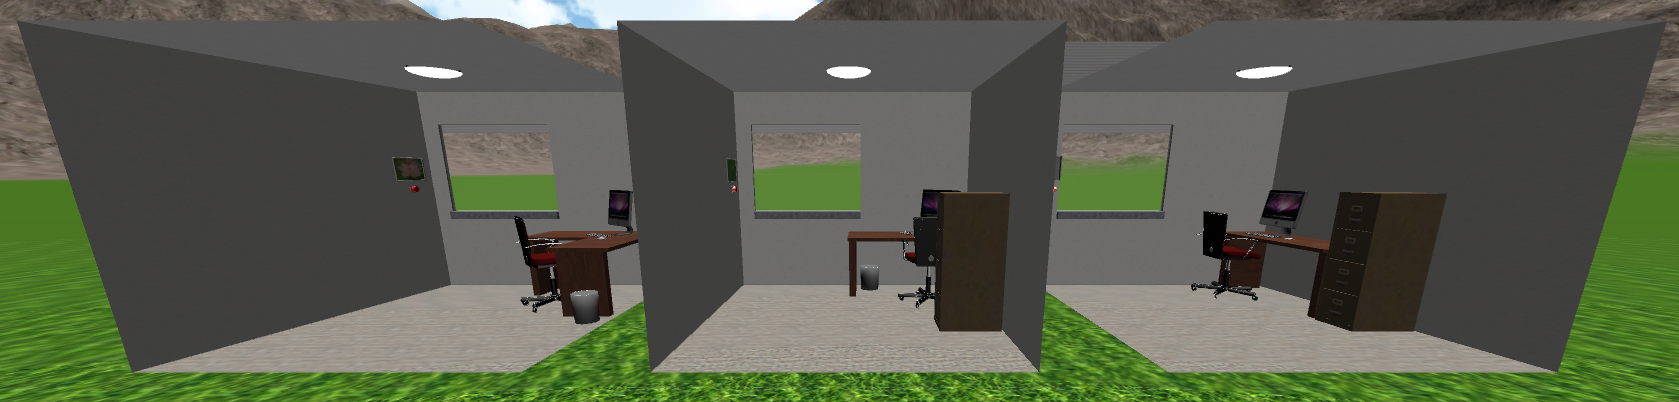
\includegraphics[width=\textwidth]{offices}
    \caption{De drie kantoren.}
    \label{fig:kantoren}
\end{figure}

Bij het betreden van de virtuele omgeving staat de proefpersoon aan het begin van
de gang, aan de rechtermuur zijn 4 deuren te zien, 80 cm breed met 80 cm er
tussen, zie Figuur \ref{fig:plan} voor een grondplan van de omgeving. Bij het 
betreden van het kantoor en het sluiten van de blinden wordt de hele gang naar 
achter verschoven zodat de deur nu aan de andere kant van de kamer staat zoals 
ge\"illustreerd in figuur \ref{fig:verandering}, na het verlaten van het kantoor 
staat de proefpersoon weer op de exacte locatie waar hij begonnen is. Wegens de 
beweging van de gang wordt er hier de illusie gecre\"eerd dat men verder in de 
gang staat dan eerst. De proefpersoon kan dan de deur van het kantoor sluiten 
om de volgende deur te openen. Dit geheel wordt drie keer herhaald. Om wat 
vari\"eteit te behouden zijn de drie kantoren, zoals ge\"illustreerd in 
figuur \ref{fig:kantoren}, lichtjes verschillend ontworpen. Enkel de knop om 
de blinden te sluiten en het fotokader er boven staat in ieder kantoor op 
dezelfde plaats.

Het grote verschil met het onderzoek van Suma et. al., 2011 \cite{suma11} is dat
de verandering in mijn omgeving veel groter is, de deur wordt volledig naar de
andere kant van de kamer verplaatst, in plaat van gewoon van hoek te veranderen.

\begin{figure}[t!]
    \centering
    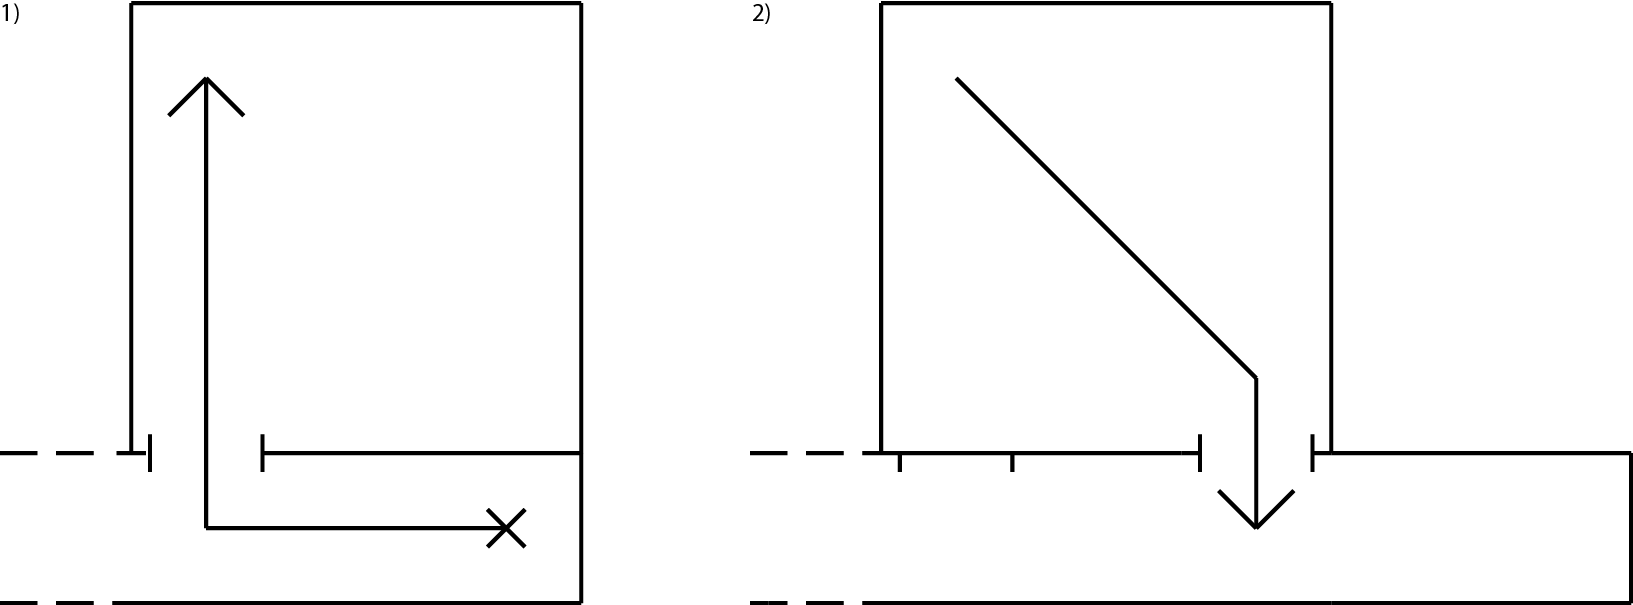
\includegraphics[width=\textwidth]{verandering}
    \caption{Verandering van de virtuele omgeving.}
    \label{fig:verandering}
\end{figure}

De beweging van de gang wordt teweeg gebracht door een transformatie in de
positie te laten gebeuren na het triggeren van de knop, wegens de implementatie
is de deur hier nooit voor in beeld. De vierde kamer dient enkel als markering 
van het einde, bij het betreden van deze kamer gaan de lichten langzaam uit.

Om een kleine hoeveelheid ruimte rondom de tracking area over te houden heb ik
hier een kleine hoeveelheid translationele vervorming toegepast (zie Paragraaf 
\ref{1:trans}), een constante factor van 1.1 op de bewegingssnelheid, daar dit 
klein genoeg is om onmerkbaar te zijn\cite{steinicke09}. Wegens de manier waarop 
dit systeem werkt is het moeilijk om een grondplan te tekenen dat overeen komt 
met de realiteit daar de kamers overlappen, in figuur \ref{fig:plan} is te zien 
wat het beoogde mentale vloerplan is van de proefpersonen.

\begin{figure}[h!]
    \centering
    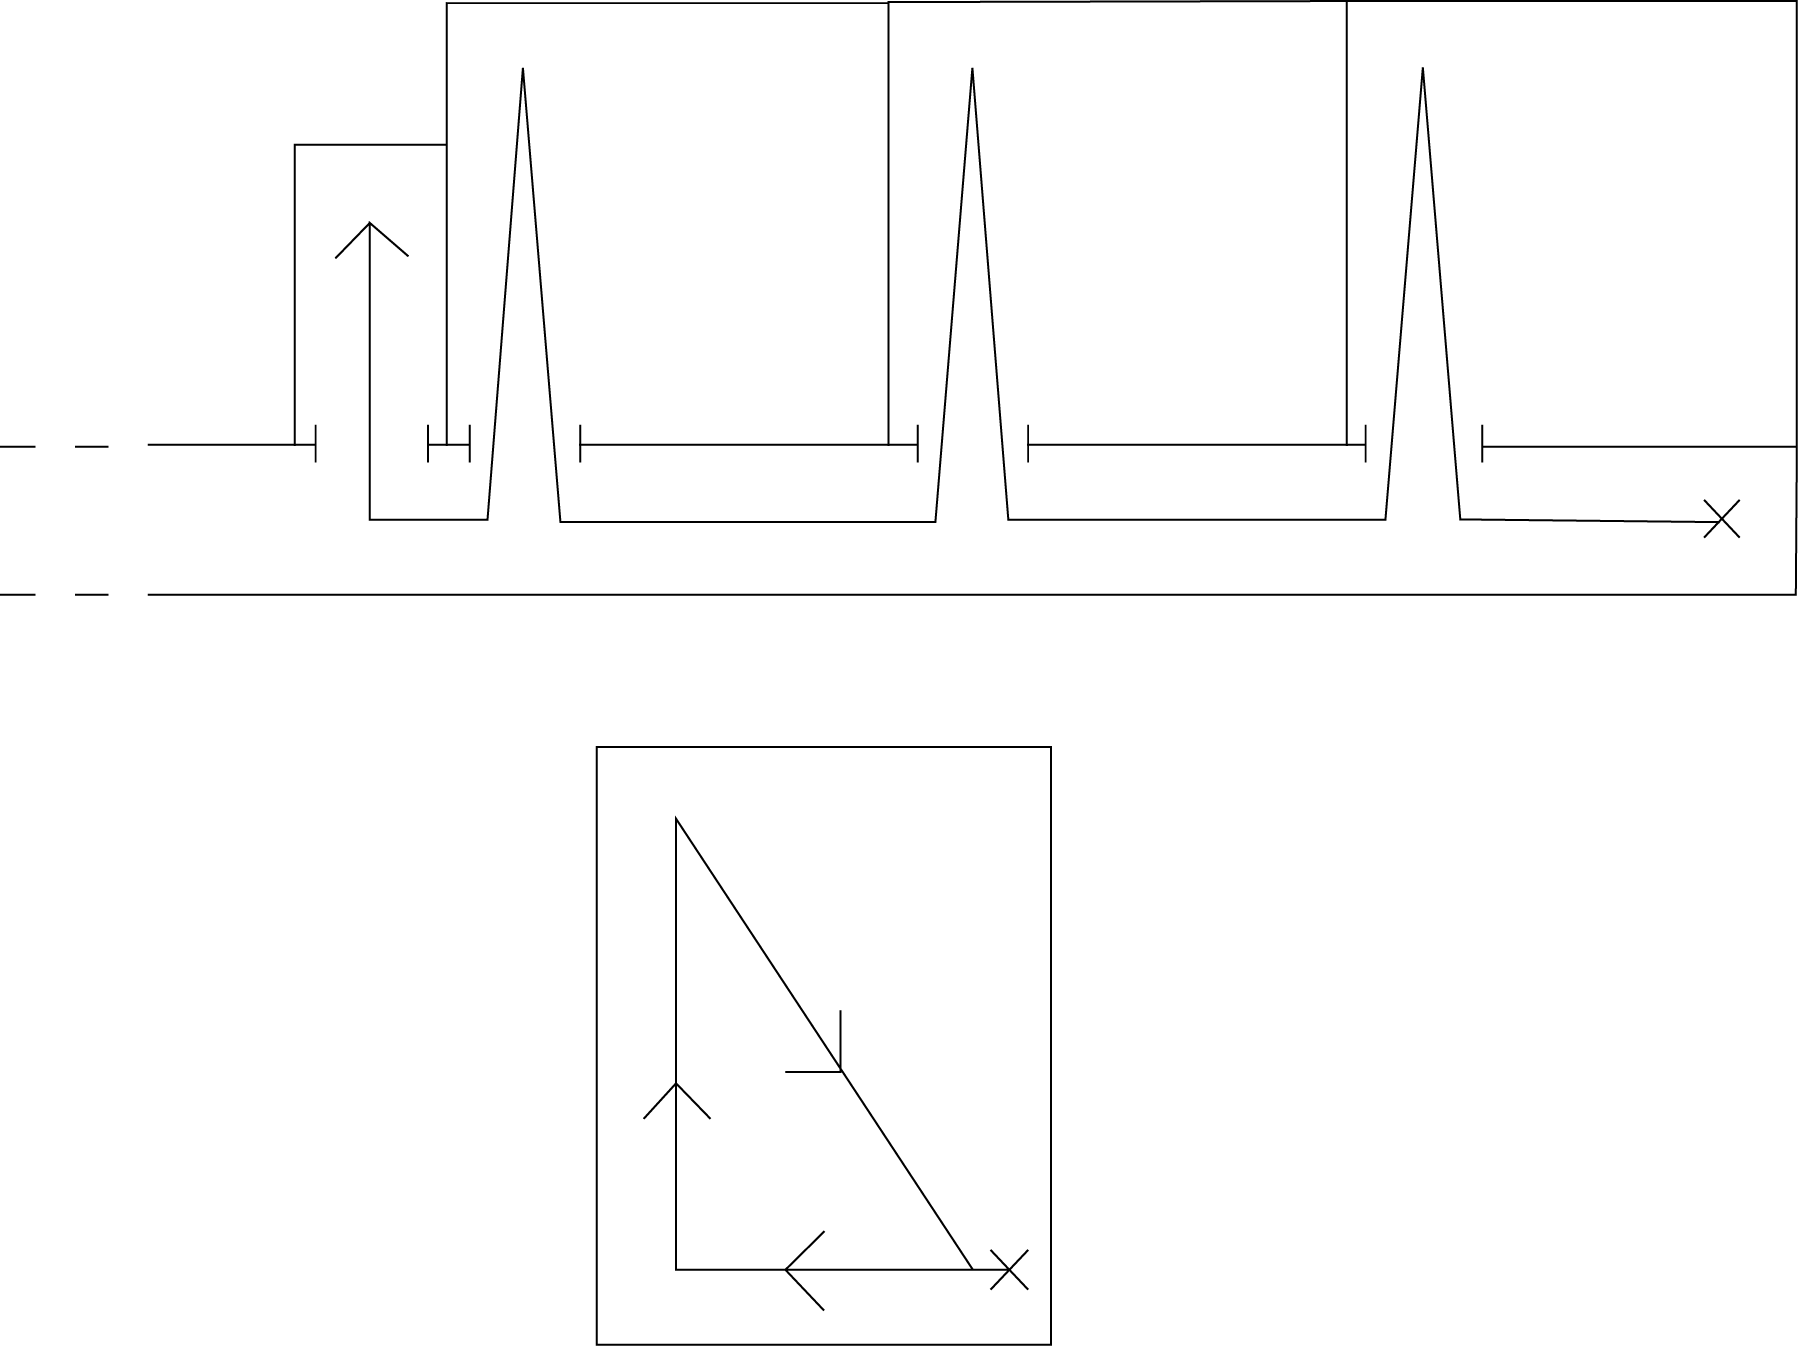
\includegraphics[width=\textwidth]{plan}
    \caption{Mentaal grondplan van de virtuele omgeving.}
    \label{fig:plan}
\end{figure}
\todo{UITBREIDEN}


\section{Pilot study}
Nadat de virtuele omgeving volledig ontworpen was, heb ik aan enkele personen
gevraagd om deze op een gewoon computerscherm met toetsenbord en muis te
doorlopen. Dit om te kijken of de implementatie functioneel in order was, en
ook om informeel te kijken hoe goed de illusie werkt. Uit deze informele studie 
is gebleken dat niemand van mijn 7 testers de redirectie merkte. Van de 7 testers
klonk er bij 4 zelfs ongeloof over mijn verklaring dat de deuren bewogen en werd
er verzocht om de omgeving nog eens te mogen doorlopen.

Ik heb hier uit geconcludeerd dat het concept zeer goed werkte, en het dus zeker
de moeite waard was om het experiment uit te breiden tot een immersief 
experiment.